\section{VOILA: Query-Conditioned Fidelity Selection}\label{sec:method}

\subsection{Problem Formulation} Let $(q, x)$ denote a visual question $q$ paired with an image $x$.
We assume access to a discrete, ordered set of input fidelities $\mathcal{F} = \{f_1, f_2, \dots, f_K\}$,
sorted by increasing acquisition cost, where each fidelity $f \in \mathcal{F}$ incurs a cost $c(f) > 0$ capturing retrieval latency, bandwidth, and compute overhead.
Lower fidelities correspond to inexpensive representations (e.g., captions or thumbnails), while higher fidelities provide richer visual information (e.g., full-resolution images).

%However, executing the VLM at multiple fidelities to empirically determine which works is prohibitively expensive at inference time.

For fidelity $f$, if the vision--language model (VLM) produces an answer $\hat{a}_f$, our objective is to select the fidelity that maximizes expected utility:
\[
f^\star
=
\arg\max_{f \in \mathcal{F}}
\underbrace{\Pr(\hat{a}_f \text{ is correct} \mid q)}_{\text{expected accuracy}} - \underbrace{\lambda c(f)}_{\text{acquisition cost}},
\]
where \textbf{the probability of correctness must be estimated \emph{without} retrieving fidelity $f$ or running the VLM at that fidelity}, and $\lambda$ controls the accuracy-cost trade-off. VOILA accomplishes this through question-conditioned learned estimators.
\fablenote{AAAI framing opportunity: this objective is a one-step value-of-information decision; say so here and cite the decision-theoretic lineage (Howard 1966, VOI; cost-sensitive feature acquisition). One sentence connecting $f^\star$ to the Bayes-optimal acquisition policy (currently hidden in Appendix theory) lifts the section from ``engineering pipeline'' to ``principled method'' --- the single highest-leverage writing change for an AAAI audience.}

%This seemingly impossible requirement---predicting VLM success without running the VLM---is what VOILA 



\subsection{Design Overview: A Three-Stage Pipeline}

VOILA adopts a three-stage pipeline: (1)~\textbf{question-conditioned success scoring} (\S\ref{sec:success_scoring}) predicts, from question features alone, how likely each fidelity is to yield a correct answer; (2)~\textbf{fidelity-specific calibration} (\S\ref{sec:voila_calibration}) converts raw scores into reliable probabilities; and (3)~\textbf{VOI selection} (\S\ref{sec:voi}) picks the minimum-cost fidelity whose expected accuracy gain justifies retrieval cost.


\subsection{Question-Conditioned Success Scoring}\label{sec:success_scoring}

%\paragraph{Motivation.} 
Fig.~\ref{fig:observations_combined} illustrates that question features contain predictive signal about cross-fidelity performance \emph{before} any visual information is retrieved. To exploit this signal, we construct training data by executing the VLM at each fidelity $f$ on labeled examples and recording whether the produced answer is correct. Let $y_f \in \{0,1\}$ denote the correctness label for fidelity $f$. We extract a question feature representation $\phi(q)$ consisting of:
\begin{itemize}[nosep]
    \item TF--IDF features of the question text (top-5{,}000 unigram vocabulary computed over the training split),
    \item lexical statistics: question length, presence of numeric tokens, superlatives, and negations,
    \item question-type indicators: five binary flags derived by rule-based matching on question-initial words and syntactic patterns (counting: \emph{how many}; yes/no: \emph{is/are/does/do}; color: \emph{what color}; spatial: \emph{where}; OCR/text: \emph{read/spell/say/written}).
\end{itemize}

We deliberately use lightweight, interpretable features rather than large pretrained encoders (e.g., BERT or sentence transformers) for two reasons.
First, it demonstrates that the task is solvable from surface-level linguistic structure alone---the central empirical claim of this paper.
Second, TF-IDF feature extraction requires no GPU and completes in under 1\,ms, making \textsc{VOILA} deployable on edge devices without a pretrained language model dependency.
The combined feature vector has 5{,}017 dimensions (5{,}000 TF-IDF + 12 lexical + 5 question-type).
Figure~\ref{fig:routing_words} (Appendix~\ref{sec:ablations}) visualizes the top-ranked TF-IDF features: words predictive of caption sufficiency (\emph{is}, \emph{there}) differ systematically from those predicting full-resolution need (\emph{color}, \emph{many}, \emph{sport}).

\fablenote{This paragraph (feature ablation + OOD transfer + vocabulary-size discussion) is results material living in the method section, and it partially duplicates \S\ref{sec:results}. Cut it to one sentence with a forward reference, and reclaim the ~12 lines for what the method section is missing: a worked end-to-end example (one real question, its features, the five calibrated probabilities, the VOI computation, the selected fidelity). A concrete trace is the fastest way for a reviewer to verify they understand the method.}
Feature ablation experiments (Table~\ref{tab:feature_ablation}, \S\ref{sec:results}) confirm that the full 5{,}017-dimensional combination achieves the best in-distribution accuracy--cost Pareto position. Crucially, question-type flags alone are competitive under cross-dataset transfer: trained on VQA-v2 and evaluated on GQA, TextVQA, and FloodNet without retraining, they retain 79--92\% of in-domain routing accuracy, whereas TF-IDF vocabulary degrades more sharply under domain shift because it encodes corpus-specific word statistics rather than language-universal syntactic roles (on FloodNet, question-type-only routing achieves 53.1\% OOD accuracy vs.\ 42.7\% for TF-IDF-only). The TF-IDF vocabulary size of 5{,}000 is a conservative high-capacity default; ablation experiments show no monotonic gain from increasing vocabulary size (performance is comparable at 1{,}000--2{,}000 tokens), so 5{,}000 is retained as a robust upper bound.

Using these features, we train a fidelity-specific regressor
\[
r_f(q) = g_f(\phi(q))
\]
to produce a raw score that correlates with the likelihood that the VLM will answer correctly at fidelity $f$. \textbf{Crucially, $g_f$ is a learned estimator of VLM behavior, not the VLM itself.} The regressor learns statistical patterns between question characteristics and cross-fidelity success rates during offline training. At inference time, \textbf{computing $r_f(q)$ requires only a forward pass through a lightweight tree ensemble---no visual retrieval, no VLM execution, no multimodal processing}. This is orders of magnitude faster and cheaper than actually running the VLM at each fidelity.



%\paragraph{Why Gradient Boosting Regressors (GBR)?}
We use a Gradient Boosting Regressor~\cite{prettenhofer2014gradient} for $g_f$: it handles high-dimensional sparse TF-IDF inputs naturally and captures non-linear question--fidelity interactions (e.g., ``counting + small objects'' $\Rightarrow$ high fidelity) without manual feature engineering. Predictor ablations (\S\ref{sec:results}) confirm calibration quality matters more than model choice; GBR, logistic regression, ridge, and MLP all perform similarly under isotonic calibration.





\subsection{Fidelity-Specific Probability Calibration}
\label{sec:voila_calibration}

%\paragraph{Motivation.}
The regressor output $r_f(q)$ is \emph{not} a calibrated probability; rather, it is a \emph{question-conditioned success score} that orders queries by their relative likelihood of being answered correctly by the vision--language model at fidelity $f$.
%Uncalibrated scores exhibit severe overlap between correct and incorrect predictions, making them unsuitable for reasoning about expected utility. Without calibration, high raw scores do not reliably indicate high success probability, leading to systematic over- or under-escalation.
Because $r_f(q)$ is not probabilistic, we apply fidelity-specific post-hoc calibration using isotonic regression~\cite{guo2017calibrationmodernneuralnetworks}.
For each fidelity $f$, we fit an isotonic regression model
\[
\psi_f: r_f(q) \mapsto \hat{p}_f(q),
\]
on a held-out 20\% split of the training data (disjoint from both GBR training and evaluation test sets), where $\hat{p}_f(q) \in [0,1]$ estimates the probability that the vision--language model would answer question $q$ correctly if executed at fidelity $f$.
All datasets are split 75\%/25\% into training and evaluation sets; within the training portion, 80\% is used for GBR training and 20\% for isotonic calibration (i.e., 60\% / 15\% / 25\% of the full dataset).
Isotonic regression is non-parametric and fits in $O(n \log n)$ time; at the dataset sizes we use (3{,}000--12{,}000 examples per fidelity), it does not require cross-validation and is not prone to overfitting. By fitting a non-decreasing mapping from raw scores to empirical success frequencies on held-out data, isotonic regression enforces monotonicity by construction and corrects systematic over- and under-confidence in the raw scores.
This calibration step uses only $(r_f(q), y_f)$ pairs, where $y_f \in \{0,1\}$ denotes historical correctness at fidelity $f$. %\paragraph{Why Isotonic Regression?}
Isotonic regression is non-parametric (no assumptions on miscalibration shape), preserves the score rank ordering learned by the regressor, and has well-understood convergence guarantees~\cite{guo2017calibrationmodernneuralnetworks} (formal bounds in Appendix~\ref{sec:calibration}).
\textbf{Cross-fidelity monotonicity.}
The per-fidelity calibrators above enforce monotonicity \emph{within} each fidelity's score-to-probability mapping, but do not guarantee that $\hat{p}_{f_1}(q) \leq \hat{p}_{f_2}(q) \leq \cdots \leq \hat{p}_{f_K}(q)$ holds \emph{across} fidelity levels for a given query.
In practice, average accuracy need not be monotone in fidelity (e.g., on TextVQA, VLM-generated captions often score higher than low-quality thumbnails because they already encode scene text).
To guarantee that the greedy escalation policy of Algorithm~\ref{alg:voila} finds the global utility optimum, we apply a lightweight secondary isotonic regression pass \emph{across} fidelity levels on the per-query calibrated scores at inference time, enforcing the ordering $\hat{p}_{f_1}(q) \leq \dots \leq \hat{p}_{f_K}(q)$.
This step adds negligible overhead ($<$0.01\,ms) and removes non-unimodal utility cases that would otherwise cause the greedy break to terminate prematurely.

\textbf{The key effect of isotonic calibration is probability reliability.}
Figure~\ref{fig:cali:scatter} shows reliability diagrams for VQA-v2/Pixtral-12B: isotonic calibration closely tracks the perfect-calibration diagonal, while raw GBR scores and VLM log-probabilities deviate substantially (ECE: 0.025\,$\to$\,0.012; Brier: 0.205\,$\to$\,0.203).
\fablenote{The Brier improvement (0.205$\to$0.203) is negligible and quoting it weakens the claim --- a careful reviewer will note that calibration barely moved Brier and ask why the paper calls calibration ``the central enabler.'' Either explain (ECE measures calibration, Brier conflates calibration with discrimination, and isotonic regression by design preserves discrimination) or drop the Brier numbers here and let the downstream routing ablation (10--25\% cost reduction) carry the argument.}
When $\hat{p}_f(q)$ reliably estimates the true correctness probability, the VOI gain $\hat{p}_{f’}(q) - \hat{p}_f(q)$ becomes an accurate predictor of the accuracy improvement from escalation.
Additional model--dataset pairs are in Appendix~\ref{sec:ablations} (Figure~\ref{fig:reliability}).

\begin{figure}[tb]
    \centering
    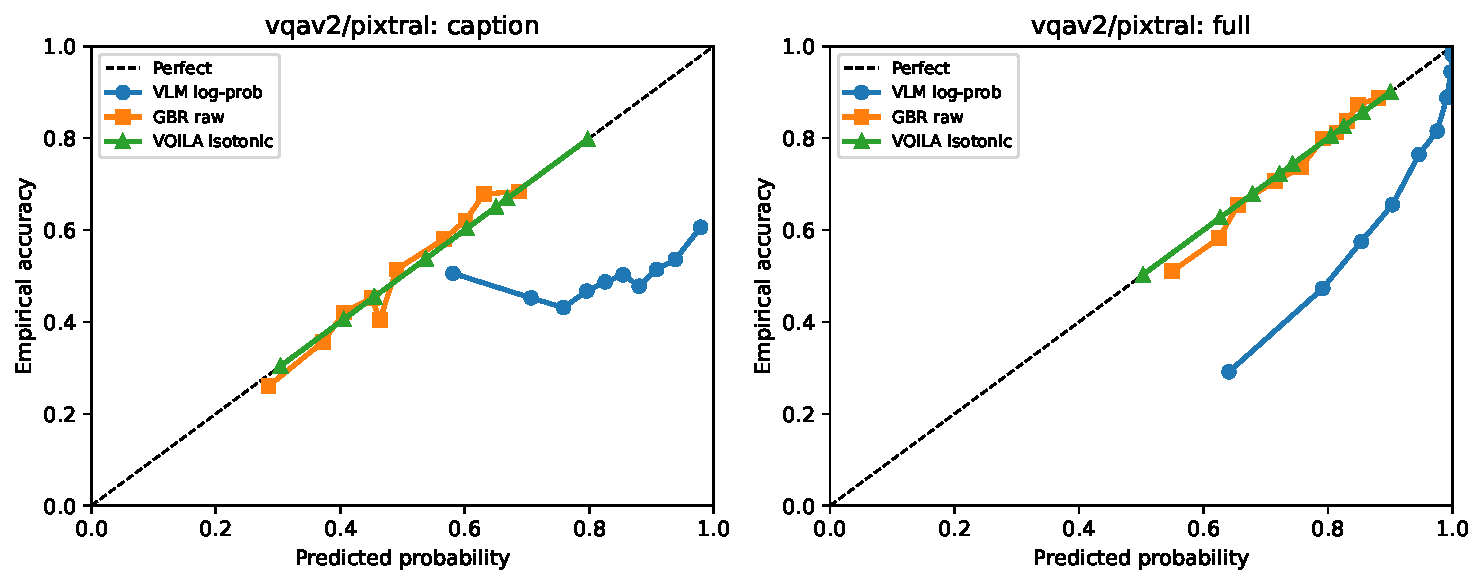
\includegraphics[width=\linewidth]{plots/reliability_vqav2_pixtral.pdf}
    \caption{\textbf{Reliability diagram} (VQA-v2, Pixtral-12B). Isotonic calibration closely tracks the perfect-calibration diagonal (dashed); raw GBR scores and VLM log-probabilities deviate substantially, causing log-prob cascades to under-escalate (Observation~2).}
    \label{fig:cali:scatter}
\end{figure}



\begin{comment}





\subsection{Fidelity-Specific Probability Calibration}\label{sec:calibration}

\begin{figure}[h]
    \centering
    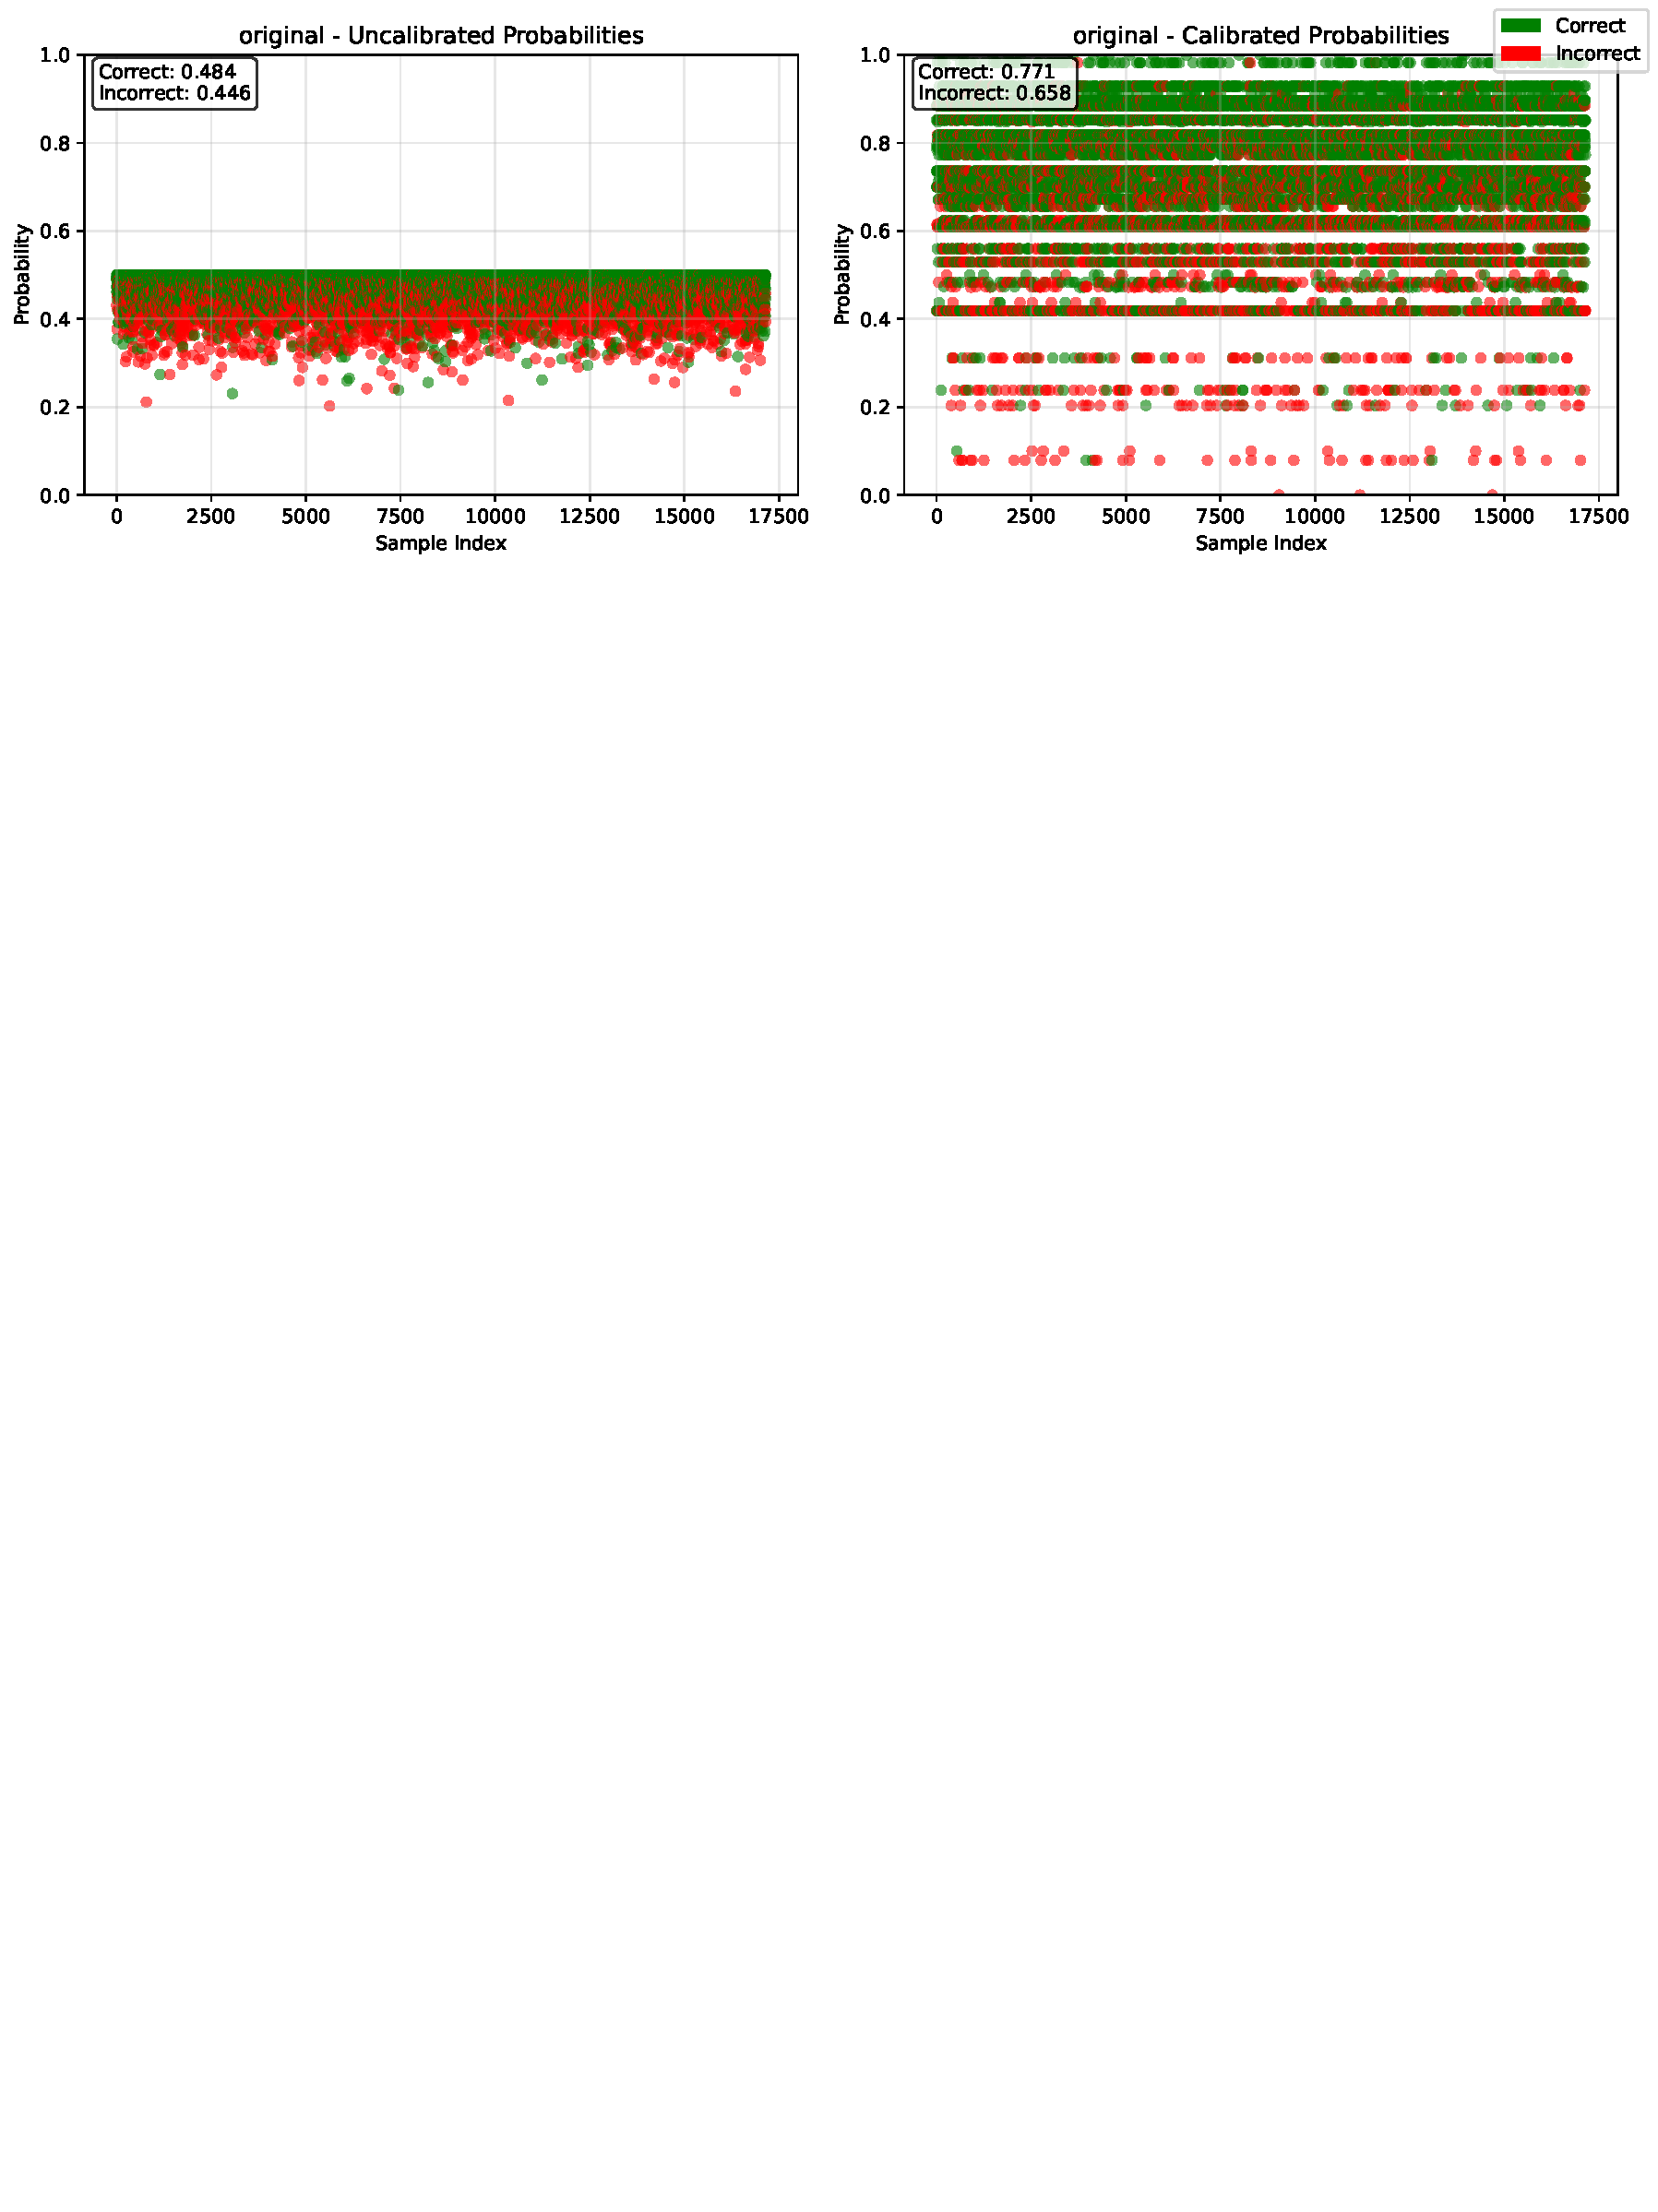
\includegraphics[width=\linewidth]{plots/calibrated_vs_uncalibrated_scatter_1.pdf}
    \caption{Calibrated vs. uncalibrated probabilities}
%Each point shows the predicted correctness probability for a query, colored by outcome.
%Uncalibrated predictors produce overlapping probabilities for correct and incorrect answers, while isotonic calibration yields well-separated, monotonic estimates that enable reliable value-of-information decisions across fidelities.}

    \label{fig:cali:scatter}
\end{figure}

The raw scores $r_f(q)$ produced by the regressor are \emph{not} calibrated probabilities. As demonstrated in Figure~\ref{fig:cali:scatter}, raw uncalibrated scores exhibit severe overlap between correct and incorrect predictions across all fidelities, making them unsuitable for reasoning about expected utility. Without calibration, high raw scores do not reliably indicate high success probability, leading to systematic over- or under-escalation. After isotonic calibration, however, the predicted probabilities become both more dispersed and better aligned with empirical correctness: correct predictions are consistently shifted toward higher probabilities, while incorrect ones are pushed downward, yielding clearer separation across caption, JPEG, and full-resolution inputs.


%\textbf{Observation 4: Calibration Enables Reliable Utility-Aware Decisions}: Figure~\ref{fig:cali:scatter} shows that raw, uncalibrated success probabilities provide little separation between correct and incorrect answers across all fidelities: predicted probabilities are tightly clustered, with substantial overlap between outcomes, making them unsuitable for reasoning about the expected benefit of escalation.  This calibrated behavior is crucial for value-of-information reasoning, as it ensures that predicted gains from acquiring higher-cost fidelities correspond to real accuracy improvements. As a result, VOILA can make stable, interpretable utility-aware decisions—escalating only when the expected benefit justifies the cost—whereas uncalibrated predictors or heuristic thresholds lack a reliable notion of marginal value and lead to inconsistent or unnecessary escalation.


%\paragraph{Motivation.}

%\paragraph{Design Decision: Isotonic Regression.}
To obtain reliable probability estimates, we apply fidelity-specific post-hoc calibration. For each fidelity $f$, we fit an isotonic regression model
\[
\psi_f: r_f(q) \mapsto \hat{p}_f(q),
\]
on a held-out calibration split, where $\hat{p}_f(q) \in [0,1]$ estimates the probability that the VLM would answer correctly at fidelity $f$.
\textbf{The key effect of calibration is separation}: isotonic regression transforms overlapping, uninformative raw scores into well-separated probabilities where correct predictions cluster near 1.0 and incorrect predictions cluster near 0.0 (Figure~\ref{fig:cali:scatter}). This separation enables VOILA to reliably distinguish queries that will succeed at low fidelity from those requiring higher fidelity---\emph{without ever running the VLM}. The calibrator learns this mapping purely from question features $\phi(q)$ and historical correctness labels $y_f$. At inference time, only the calibrated predictor $\hat{p}_f(q)$ is used; no additional calibration or model execution is required.

%\paragraph{Why Isotonic Regression?}
Isotonic regression offers VOILA three critical properties, when compared to other calibration techniques:
\begin{enumerate}[nosep]
    \item \textbf{Monotonicity preservation}: Ensures that higher raw scores always map to higher probabilities, maintaining the rank ordering learned by the regressor.
    \item \textbf{Non-parametric}: Makes no assumptions about the functional form of miscalibration, allowing it to correct arbitrary systematic biases.
    \item \textbf{Proven calibration guarantees}: Isotonic regression is a standard tool in probability calibration with well-understood convergence properties.
\end{enumerate}

%As shown in Figure~\ref{fig:cali:scatter}, isotonic calibration transforms overlapping, uninformative score distributions into well-separated, reliable probabilities that enable stable value-of-information reasoning. 


\end{comment}


\subsection{Value-of-Information--Based Fidelity Selection}
\label{sec:voi}

%\paragraph{Motivation.}
With calibrated success probabilities $\hat{p}_f(q)$ in hand---\textbf{computed from question features alone, without any VLM execution}---we can now reason explicitly about the \emph{marginal value} of acquiring higher-cost fidelities. The key insight is that we should escalate to a more expensive representation only when the expected improvement in accuracy justifies the additional acquisition cost.
%\paragraph{Design Decision: Greedy VOI Escalation.}

Starting from the lowest-cost fidelity $f_1$, VOILA evaluates whether escalating to the next higher fidelity $f_j$ is beneficial by computing the \textbf{Value of Information (VOI)}:
\[
\mathrm{VOI}(f_j \mid f_i)
=
\underbrace{[\hat{p}_{f_j}(q) - \hat{p}_{f_i}(q)]}_{\text{expected accuracy gain}} - \underbrace{\lambda c(f_j)}_{\text{acquisition cost}}.
\]

\textsc{VOILA} incrementally increases fidelity only when $\mathrm{VOI}(f_j \mid f_i) > \tau$, i.e., when the expected improvement in correctness outweighs the additional acquisition cost, where $\tau$ is a decision threshold and $\lambda$ is a cost penalty.
Both $\lambda$ and $\tau$ are tuned by grid search on the validation split of each training dataset; $\tau = 0$ (escalate whenever expected gain exceeds cost) serves as a strong default, and \textsc{VOILA} is robust to moderate changes in $\lambda$ because it depends only on relative cost differences between fidelities (full sensitivity analysis in Appendix~\ref{sec:reproducibility}).
The greedy policy requires only $K$ forward passes through the calibrated predictors (no tree search), is near-optimal under the diminishing-returns assumption (Corollary~1, Appendix~\ref{sec:regret}), and exposes the interpretable cost-tradeoff knobs $\lambda$ and $\tau$.

\begin{algorithm}[tb]
\caption{\textsc{VOILA} Inference Procedure}
\label{alg:voila}
\small
\begin{algorithmic}[1]
\State \textbf{Input:} Query $q$, fidelity set $\mathcal{F}=\{f_1,\ldots,f_K\}$, $\lambda$, $\tau$
\State \textbf{Output:} Selected fidelity $f^*$ and answer $\hat{a}_{f^*}$
\State $f \gets f_1$;\; $\hat{p} \gets \psi_{f_1}(r_{f_1}(q))$ \hfill\Comment{no image, no VLM}
\For{$f' \in \{f_2, \ldots, f_K\}$ in ascending cost order}
    \State $\hat{p}' \gets \psi_{f'}(r_{f'}(q))$
    \If{$(\hat{p}' - \hat{p}) - \lambda c(f') > \tau$}
        \State $f \gets f'$;\; $\hat{p} \gets \hat{p}'$
    \Else\; \textbf{break}
    \EndIf
\EndFor
\State Retrieve image at fidelity $f$; run VLM; \Return $f,\hat{a}_f$
\end{algorithmic}
\end{algorithm}

\textsc{VOILA} requires no modifications to the underlying VLM; it is compatible with any model that produces discrete correctness labels for offline training. The GBR predictor and isotonic calibrator are trained per VLM on 3,000--12,000 labeled examples per fidelity (minutes on standard hardware), then used at inference time to select the optimal fidelity from question text alone before any visual data is accessed.


%In this section, we describe the design and core algorithms of \textbf{VOILA} (\underline{V}alue-\underline{O}f-\underline{I}nformation guided \underline{L}atency-\underline{A}ware fidelity selection).



%, a query-adaptive framework for selecting the minimum-cost input fidelity required to answer a multimodal query accurately, using \emph{only} features of the question text—\emph{before} retrieving any visual input or executing a vision--language model (VLM).
%While VLMs expose token-level confidence scores after inference, these signals are fundamentally unsuitable for fidelity selection.
%As shown in Figures~\ref{fig:observations_combined} and~\ref{fig:cali:scatter}, VLM confidence exhibits substantial overlap between correct and incorrect predictions when visual information is insufficient, frequently producing confident but incorrect answers at low fidelity.
%Crucially, such confidence scores are available only \emph{after} visual retrieval and model execution, rendering them unusable for pre-retrieval decision-making.



%The key design principle underlying VOILA is simple: \emph{different queries have different minimum information requirements, and these requirements are predictable from the question alone---without ever executing the VLM or retrieving visual content at inference time}.

%\subsection{The Core Challenge: Pre-Retrieval Decision-Making}


%Consider the motivating example from Figure~1: given the query ``Which airline is this plane from?'', we must decide whether to retrieve a caption (2KB), a low-resolution thumbnail (9KB), a compressed image (46KB), or the full-resolution original (433KB) \emph{before} incurring any retrieval or processing costs. This decision must be made using only the question text, as accessing visual content to ``check'' which fidelity works would defeat the purpose of adaptive selection.

%This \textbf{pre-retrieval constraint} distinguishes our problem from existing model routing approaches, which assume all context is freely available and optimize only \emph{which model} to apply. In contrast, VOILA optimizes \emph{which representation of the context to acquire} before any expensive operations occur. \textbf{Critically, VOILA never executes the VLM to determine fidelity selection at inference time}---all predictions are made from question features alone, using lightweight learned estimators trained offline.
